% Options for packages loaded elsewhere
\PassOptionsToPackage{unicode}{hyperref}
\PassOptionsToPackage{hyphens}{url}
%
\documentclass[
]{article}
\usepackage{amsmath,amssymb}
\usepackage{iftex}
\ifPDFTeX
  \usepackage[T1]{fontenc}
  \usepackage[utf8]{inputenc}
  \usepackage{textcomp} % provide euro and other symbols
\else % if luatex or xetex
  \usepackage{unicode-math} % this also loads fontspec
  \defaultfontfeatures{Scale=MatchLowercase}
  \defaultfontfeatures[\rmfamily]{Ligatures=TeX,Scale=1}
\fi
\usepackage{lmodern}
\ifPDFTeX\else
  % xetex/luatex font selection
\fi
% Use upquote if available, for straight quotes in verbatim environments
\IfFileExists{upquote.sty}{\usepackage{upquote}}{}
\IfFileExists{microtype.sty}{% use microtype if available
  \usepackage[]{microtype}
  \UseMicrotypeSet[protrusion]{basicmath} % disable protrusion for tt fonts
}{}
\makeatletter
\@ifundefined{KOMAClassName}{% if non-KOMA class
  \IfFileExists{parskip.sty}{%
    \usepackage{parskip}
  }{% else
    \setlength{\parindent}{0pt}
    \setlength{\parskip}{6pt plus 2pt minus 1pt}}
}{% if KOMA class
  \KOMAoptions{parskip=half}}
\makeatother
\usepackage{xcolor}
\usepackage[margin=1in]{geometry}
\usepackage{graphicx}
\makeatletter
\def\maxwidth{\ifdim\Gin@nat@width>\linewidth\linewidth\else\Gin@nat@width\fi}
\def\maxheight{\ifdim\Gin@nat@height>\textheight\textheight\else\Gin@nat@height\fi}
\makeatother
% Scale images if necessary, so that they will not overflow the page
% margins by default, and it is still possible to overwrite the defaults
% using explicit options in \includegraphics[width, height, ...]{}
\setkeys{Gin}{width=\maxwidth,height=\maxheight,keepaspectratio}
% Set default figure placement to htbp
\makeatletter
\def\fps@figure{htbp}
\makeatother
\setlength{\emergencystretch}{3em} % prevent overfull lines
\providecommand{\tightlist}{%
  \setlength{\itemsep}{0pt}\setlength{\parskip}{0pt}}
\setcounter{secnumdepth}{-\maxdimen} % remove section numbering
\usepackage{booktabs}
\usepackage{longtable}
\usepackage{array}
\usepackage{multirow}
\usepackage{wrapfig}
\usepackage{float}
\usepackage{colortbl}
\usepackage{pdflscape}
\usepackage{tabu}
\usepackage{threeparttable}
\usepackage{threeparttablex}
\usepackage[normalem]{ulem}
\usepackage{makecell}
\usepackage{xcolor}
\ifLuaTeX
  \usepackage{selnolig}  % disable illegal ligatures
\fi
\usepackage{bookmark}
\IfFileExists{xurl.sty}{\usepackage{xurl}}{} % add URL line breaks if available
\urlstyle{same}
\hypersetup{
  pdftitle={An Analysis on Key Factors that Influence Suicide Rates},
  pdfauthor={Cynthia Luo},
  hidelinks,
  pdfcreator={LaTeX via pandoc}}

\title{An Analysis on Key Factors that Influence Suicide Rates}
\author{Cynthia Luo}
\date{}

\begin{document}
\maketitle

\hfill\break

\textbf{Source Code on GitHub:}
\url{https://github.com/bluenut15/JSC370-project-web.git}

\hfill\break

\section{Introduction}\label{introduction}

Suicide is a pressing global public health issue, with profound social,
economic, and psychological implications. Understanding the factors that
contribute to suicide rates is essential for shaping effective
prevention strategies and informing targeted interventions. While much
prior research has explored economic and social influences on mental
health outcomes, the relationship between macro-level indicators---such
as income inequality, national wealth, and health system
investment---and suicide rates remains complex and often varies by
region.

This, this study aims to investigate the research questions: What are
the key factors that influence suicide rates and how do they influence
suicide rates? Do the relationships differ across regions around the
world?

To explore these questions, I constructed a comprehensive dataset with a
response (suicide rates) and main predictors (annual GDP per capita of
countries, annual Gini index of countries, annual health spending
percentage of countries, region of countries) by merging four different
data sources. The suicide rates dataset, retrieved from the World Health
Organization (WHO) API, provides annual crude suicide rates per 100,000
population for countries from 2000 to 2021. The health expenditure
dataset, also obtained through the WHO API, contains information on
health spending as a percentage of GDP across countries from 2000 to
2022 (``The Global Health Observatory'', 2025). Economic indicators were
sourced from Our World in Data, which compiles data from the World Bank.
The GDP per capita dataset includes annual per capita income in
international dollars for various countries from 1990 to 2023 (``GDP per
capita'', 2025), while the Gini index dataset provides yearly measures
of income inequality for various countries from 1963 to 2023 (``Gini
Coefficient'', 2024). By merging these four datasets based on region,
country code, and year, I created a unified dataset that allows for a
more thorough analysis of the factors associated with suicide rates.
Exploratory figures and plots, as well as regression analysis, were
employed to investigate the research questions.

\hfill\break
\hfill\break

\section{Methods}\label{methods}

The data for this analysis was obtained from multiple sources using API
queries and online databases. The suicide rates data was retrieved from
the World Health Organization (WHO) API, providing annual crude suicide
rates per 100,000 population for 185 countries around the world from
2000 to 2021. The API response was filtered to include only aggregate
data for both sexes and all age groups. The health expenditure data was
also extracted from the WHO API, containing annual health expenditure as
a percentage of GDP for 194 countries from 2000 to 2022. In addition to
the numerical variables of interest, the two WHO datasets also have
information on the parent location, or region, of each country. The GDP
per capita data was downloaded from Our World in Data, which sourced the
dataset from the World Bank's World Development Indicators in 2025. The
dataset contains the annual GDP per capita of all countries worldwide
from 1990 to 2023. The Gini index data was downloaded from Our World in
Data, with data originally retrieved from the World Bank's Poverty and
Inequality Platform in 2024. This dataset provides the annual Gini
coefficient for 170 countries from 1963 to 2023.

To clean the datasets appropriately, I first explored the four datasets
to understand their structure and identify missing or abnormal values.
Then, in the Gini index dataset, I dropped an irrelevant column
containing only missing values. Afterward, I removed all rows with any
missing values from all datasets to ensure completeness. After cleaning,
I merged the four datasets using an inner join on common columns:
country, year, and region. This ensured that only observations with
complete information across all variables were retained. Lastly, I
removed a duplicate country name column and renamed the remaining
variables for GDP per capita, Gini index, and country name to improve
readability in the final merged dataset.

The data analysis began with creating a summary statistics table that
presented the mean, median, standard deviation, minimum, and maximum
values for key numerical variables (suicide rate, GDP per capita, Gini
index, and health spending). This provided an initial overview of the
central tendency and variability in the dataset. Next, I visualized the
distributions of all key variables (suicide rate, GDP per capita, Gini
index, health spending, and region) using histograms and bar plots, and
examined the relationships between the predictors (GDP per capita, Gini
index, health spending, and region) and suicide rates through
scatterplots and box plots. During this exploratory phase, I observed
evidence of a non-linear relationship between suicide rates and the
numerical predictors, which motivated the transformation of the response
variable. Specifically, I applied a square root transformation to
suicide rates to improve linearity and model fit. To further investigate
patterns and relationships, I employed linear regression analysis, which
models the relationship between a dependent variable and one or more
independent variables by fitting a linear equation to the observed data.
I fitted and compared three linear regression models:

\begin{itemize}
\item
  Model 0: A baseline model using the untransformed suicide rates and
  the numerical predictors GDP per capita, Gini index, and health
  spending.
\item
  Model 1: A transformed model using the square root of suicide rates as
  the response variable, with the same predictors as Model 0.
\item
  Model 2: An extended model using the square root of suicide rates as
  the response variable, all the key predictors GDP per capita, Gini
  index, health spending, and region, but also incorporating interaction
  terms between each numerical predictor and region to account for
  regional variation in effects.
\end{itemize}

Predictor significance in each model was evaluated using t-test
p-values, with the threshold being 0.05. The performance of each model
was evaluated using RSS, R squared, adjusted R squared, and overall
F-test p-values.

\hfill\break
\hfill\break

\section{Results}\label{results}

The final merged dataset contained 1,567 observations on 8 variables:
year, suicide rates, GDP per capita, Gini index, health spending
percentage, region, country code, and country name, for 156 countries
around the world. Exploratory data analysis as well as regression
analysis were employed to explore the data and investigate the research
question.

\newpage

\begingroup\fontsize{10}{12}\selectfont

\begin{longtable}[t]{lrrrrr}
\toprule
\textbf{Variable} & \textbf{Mean} & \textbf{Median} & \textbf{SD} & \textbf{Min} & \textbf{Max}\\
\midrule
\endfirsthead
\multicolumn{6}{@{}l}{\textit{(continued)}}\\
\toprule
\textbf{Variable} & \textbf{Mean} & \textbf{Median} & \textbf{SD} & \textbf{Min} & \textbf{Max}\\
\midrule
\endhead

\endfoot
\bottomrule
\endlastfoot
\cellcolor[HTML]{f5f5f5}{Suicide Rate (per 100,000)} & \cellcolor[HTML]{f5f5f5}{11.292} & \cellcolor[HTML]{f5f5f5}{9.392} & \cellcolor[HTML]{f5f5f5}{8.083} & \cellcolor[HTML]{f5f5f5}{0.085} & \cellcolor[HTML]{f5f5f5}{53.058}\\
GDP per Capita (international dollars) & 28878.138 & 21822.988 & 24218.310 & 833.920 & 140435.800\\
\cellcolor[HTML]{f5f5f5}{Gini Index} & \cellcolor[HTML]{f5f5f5}{0.369} & \cellcolor[HTML]{f5f5f5}{0.351} & \cellcolor[HTML]{f5f5f5}{0.083} & \cellcolor[HTML]{f5f5f5}{0.232} & \cellcolor[HTML]{f5f5f5}{0.648}\\
Health Spending (\% of GDP) & 7.050 & 6.959 & 2.545 & 1.718 & 18.813\\*
\end{longtable}
\endgroup{}

\textbf{Table 1:} Summary statistics for key numerical variables,
including suicide rate, GDP per capita, Gini index, and health spending.
Values shown include the mean, median, standard deviation, minimum, and
maximum across all countries and years in the dataset.

\hfill\break

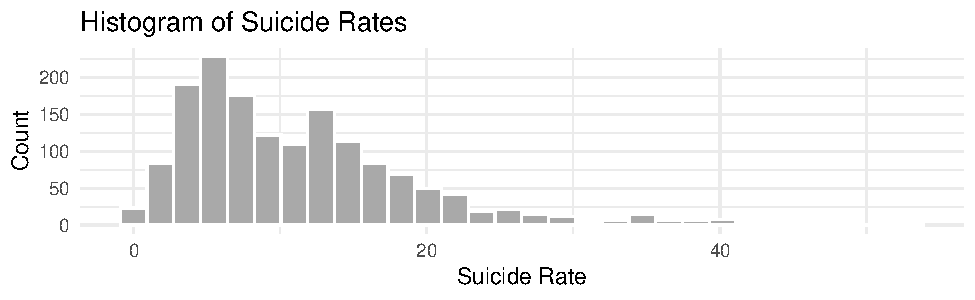
\includegraphics{final_report_files/figure-latex/variable-distributions-1.pdf}
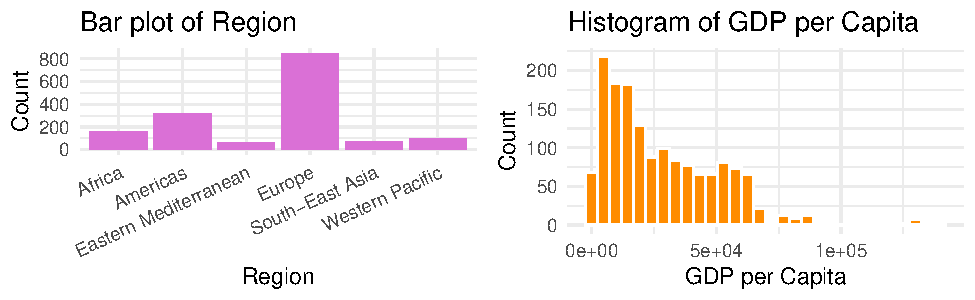
\includegraphics{final_report_files/figure-latex/variable-distributions-2.pdf}
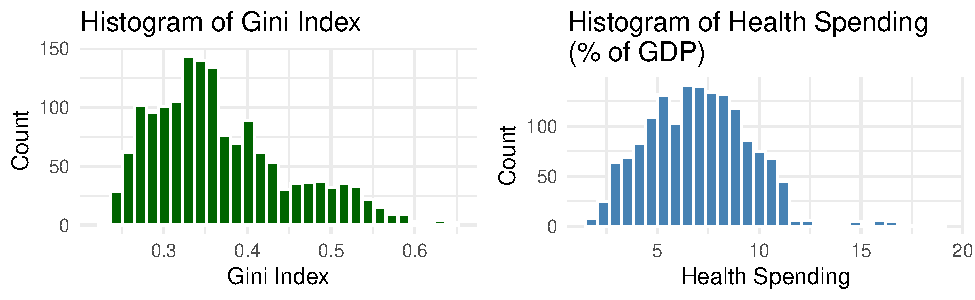
\includegraphics{final_report_files/figure-latex/variable-distributions-3.pdf}

\textbf{Figure 1:} Distribution of key variables in the dataset,
including that for suicide rates (top plot), region (middle left plot),
GDP per capita (middle right plot), Gini index (bottom left plot), and
health spending as a percentage of GDP (bottom right plot).

\newpage

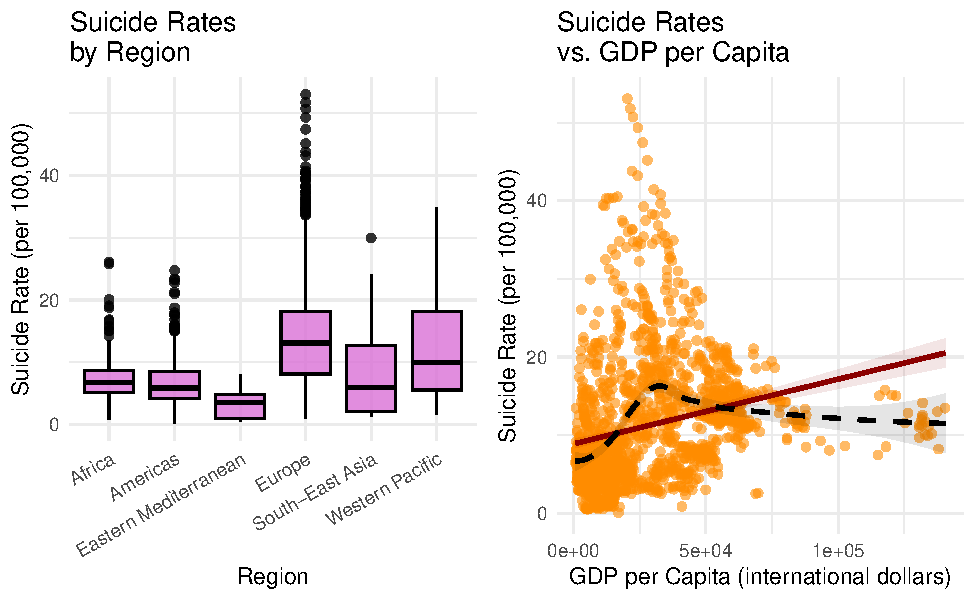
\includegraphics{final_report_files/figure-latex/suicide-against-vars-1.pdf}
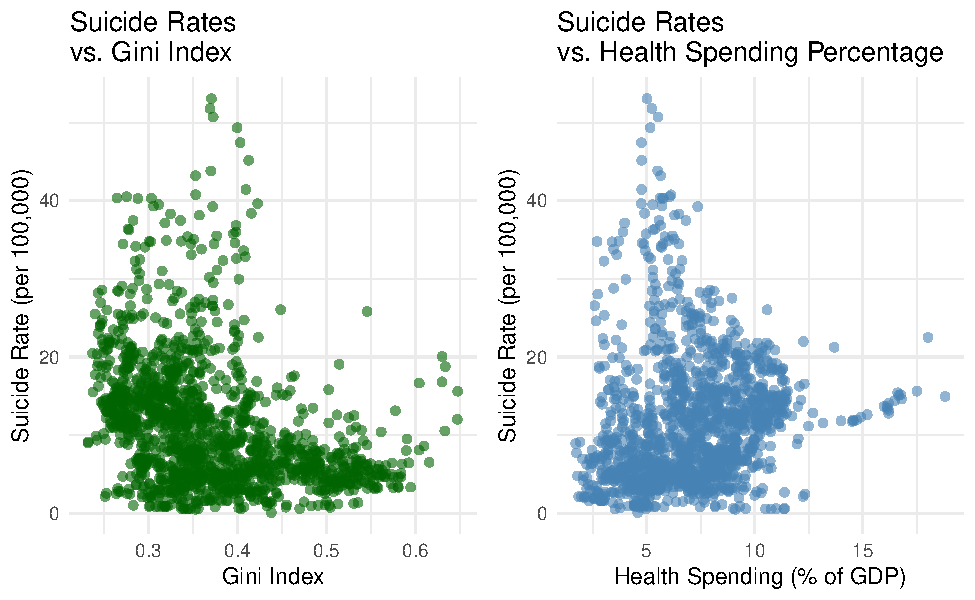
\includegraphics{final_report_files/figure-latex/suicide-against-vars-2.pdf}

\textbf{Figure 2:} Relationship between suicide rates and key
predictors, including region (top left plot), GDP per capita (top right
plot), Gini index (bottom left plot), and health spending as a
percentage of GDP (bottom right plot).

\newpage

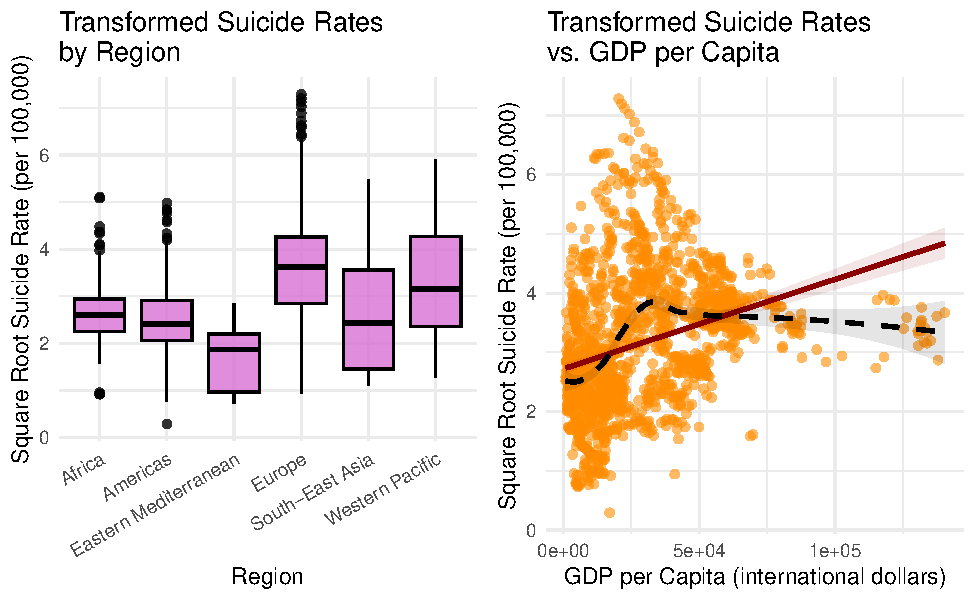
\includegraphics{final_report_files/figure-latex/suicide-against-numeric-transformed-1.pdf}
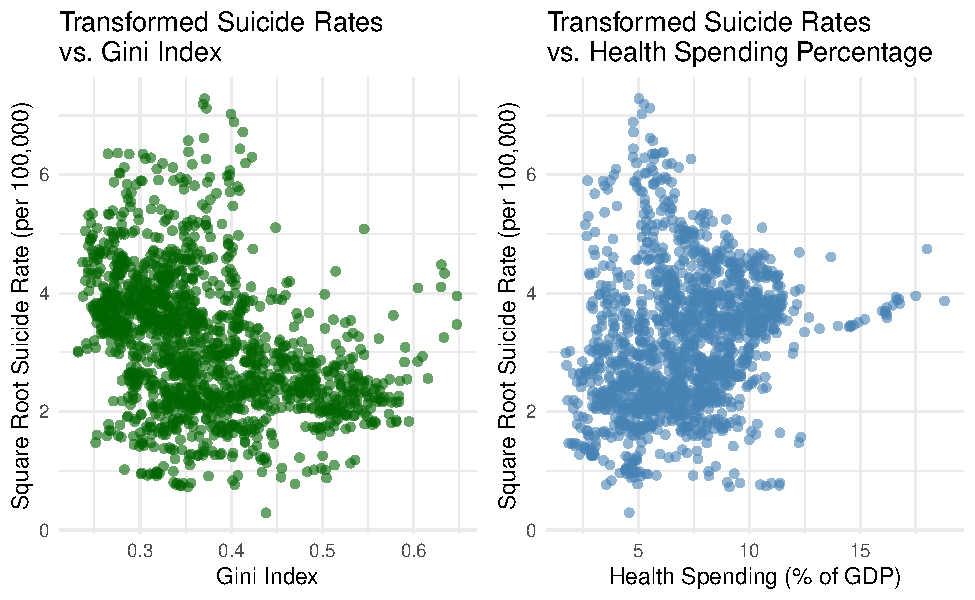
\includegraphics{final_report_files/figure-latex/suicide-against-numeric-transformed-2.pdf}

\textbf{Figure 3:} Relationship between square root-transformed suicide
rates and key predictors, including region (top left plot), GDP per
capita (top right plot), Gini index (bottom left plot), and health
spending as a percentage of GDP (bottom right plot).

\newpage

Table 1 summarizes the distribution of key numerical variables across
all countries and years in the dataset. On average, the suicide rate is
approximately 11.292 per 100,000 people, with a standard deviation of
8.083, ranging from 0.085 to 53.058. GDP per capita has a wide range,
with a mean of approximately \$28,878, but a maximum exceeding
\$140,000, indicating substantial variation in income levels across
countries. The Gini index, a measure of income inequality, has a mean
value of approximately 0.369, suggesting moderate inequality overall,
with relatively low standard deviation of 0.083. Health spending as a
percentage of GDP averages around 7.05\%, with values spanning from
1.718\% to 18.813\%, reflecting differing national priorities and
capacities for healthcare investment.

Figure 1 showcases patterns in each variable's distribution. Suicide
rates are right-skewed, with most values concentrated below 20 per
100,000 and a long tail extending toward higher rates. The regional
distribution is imbalanced, with Europe contributing the largest number
of observations, and the Eastern Mediterranean, South-East Asia, and
Western Pacific contributing much fewer. GDP per capita is right-skewed,
with a majority of countries clustered at lower income levels and a
small number exhibiting extremely high values. Similarly, the Gini index
is also right-skewed. In contrast, the health spending as a percentage
of GDP is approximately symmetric and bell-shaped, peaking around 7 to
8\%, though a few countries spend significantly more.

Figure 2 illustrates the relationships between suicide rates and key
predictors. For region, Europe and Western Pacific regions show higher
median suicide rates than other regions. For the numeric predictors,
there appears to be a non-linear negative association between suicide
rates and GDP per capita, Gini index, and health spending percentage.
These curved patterns suggest that the assumptions of linearity and
constant variance may not hold in a basic linear regression model. To
address this, a square root transformation was applied to the suicide
rate variable, as shown in Figure 3. The transformed plots exhibit more
stabilized variance and improved linearity in the relationships,
particularly with GDP per capita and Gini index. However, the
transformed relationships still display some degree of
curvature---especially for GDP per capita and health spending
percentage---indicating that while the transformation improves model
fit, it does not fully resolve non-linearity, likely due to skewness or
the presence of outliers in the data.

Building on the insights from the exploratory analysis, I proceeded to
conduct regression analysis to formally assess the influence of each
predictor on suicide rates as well as the performance of each model fit:

\begin{itemize}
\item
  Model 0: A baseline model using the untransformed suicide rates and
  the numerical predictors GDP per capita, Gini index, and health
  spending.
\item
  Model 1: A transformed model using the square root of suicide rates as
  the response variable, with the same predictors as Model 0.
\item
  Model 2: An extended model using the square root of suicide rates as
  the response variable, all the key predictors GDP per capita, Gini
  index, health spending, and region, but also incorporating interaction
  terms between each numerical predictor and region to account for
  regional variation in effects.
\end{itemize}

This allowed for a more rigorous evaluation of the relationships between
suicide rates and the predictors.

\newpage

\begingroup\fontsize{10}{12}\selectfont

\begin{longtable}[t]{lrrrr}
\toprule
\textbf{Term} & \textbf{Estimate} & \textbf{Std. Error} & \textbf{t value} & \textbf{t-Test p-value}\\
\midrule
\endfirsthead
\multicolumn{5}{@{}l}{\textit{(continued)}}\\
\toprule
\textbf{Term} & \textbf{Estimate} & \textbf{Std. Error} & \textbf{t value} & \textbf{t-Test p-value}\\
\midrule
\endhead

\endfoot
\bottomrule
\endlastfoot
\cellcolor[HTML]{f5f5f5}{Intercept} & \cellcolor[HTML]{f5f5f5}{20.751} & \cellcolor[HTML]{f5f5f5}{1.190} & \cellcolor[HTML]{f5f5f5}{17.443} & \cellcolor[HTML]{f5f5f5}{0.000}\\
GDP per Capita & 0.000 & 0.000 & 3.396 & 0.001\\
\cellcolor[HTML]{f5f5f5}{Gini Index} & \cellcolor[HTML]{f5f5f5}{-29.751} & \cellcolor[HTML]{f5f5f5}{2.572} & \cellcolor[HTML]{f5f5f5}{-11.566} & \cellcolor[HTML]{f5f5f5}{0.000}\\
Health Spending & 0.078 & 0.086 & 0.902 & 0.367\\*
\end{longtable}
\endgroup{}

\textbf{Table 2.1:} Coefficient summary table for Model 0, which models
untransformed suicide rates using GDP per capita, Gini index, and health
spending as predictors. The table presents coefficient estimates,
standard errors, t-values, and associated p-values for each term in the
model.

\hfill\break

\begingroup\fontsize{10}{12}\selectfont

\begin{longtable}[t]{lr}
\toprule
\textbf{Metric} & \textbf{Value}\\
\midrule
\endfirsthead
\multicolumn{2}{@{}l}{\textit{(continued)}}\\
\toprule
\textbf{Metric} & \textbf{Value}\\
\midrule
\endhead

\endfoot
\bottomrule
\endlastfoot
\cellcolor[HTML]{f5f5f5}{Residual Sum of Squares (RSS)} & \cellcolor[HTML]{f5f5f5}{88435.973}\\
R-squared & 0.136\\
\cellcolor[HTML]{f5f5f5}{Adjusted R-squared} & \cellcolor[HTML]{f5f5f5}{0.134}\\
Overall F-test p-value & 0.000\\*
\end{longtable}
\endgroup{}

\textbf{Table 2.2:} Performance metrics for Model 0, including \(RSS\),
\(R^2\), adjusted \(R^2\), and overall F-test p-value. These metrics
reflect the model's ability to explain variation in suicide rates across
observations.

\hfill\break
\hfill\break

\begingroup\fontsize{10}{12}\selectfont

\begin{longtable}[t]{lrrrr}
\toprule
\textbf{Term} & \textbf{Estimate} & \textbf{Std. Error} & \textbf{t value} & \textbf{t-Test p-value}\\
\midrule
\endfirsthead
\multicolumn{5}{@{}l}{\textit{(continued)}}\\
\toprule
\textbf{Term} & \textbf{Estimate} & \textbf{Std. Error} & \textbf{t value} & \textbf{t-Test p-value}\\
\midrule
\endhead

\endfoot
\bottomrule
\endlastfoot
\cellcolor[HTML]{f5f5f5}{Intercept} & \cellcolor[HTML]{f5f5f5}{4.250} & \cellcolor[HTML]{f5f5f5}{0.165} & \cellcolor[HTML]{f5f5f5}{25.769} & \cellcolor[HTML]{f5f5f5}{0.000}\\
GDP per Capita & 0.000 & 0.000 & 5.245 & 0.000\\
\cellcolor[HTML]{f5f5f5}{Gini Index} & \cellcolor[HTML]{f5f5f5}{-4.124} & \cellcolor[HTML]{f5f5f5}{0.357} & \cellcolor[HTML]{f5f5f5}{-11.567} & \cellcolor[HTML]{f5f5f5}{0.000}\\
Health Spending & 0.032 & 0.012 & 2.651 & 0.008\\*
\end{longtable}
\endgroup{}

\textbf{Table 3.1:} Coefficient summary table for Model 1, which models
square root-transformed suicide rates using GDP per capita, Gini index,
and health spending as predictors. The table presents coefficient
estimates, standard errors, t-values, and associated p-values for each
term in the model.

\hfill\break

\begingroup\fontsize{10}{12}\selectfont

\begin{longtable}[t]{lr}
\toprule
\textbf{Metric} & \textbf{Value}\\
\midrule
\endfirsthead
\multicolumn{2}{@{}l}{\textit{(continued)}}\\
\toprule
\textbf{Metric} & \textbf{Value}\\
\midrule
\endhead

\endfoot
\bottomrule
\endlastfoot
\cellcolor[HTML]{f5f5f5}{Residual Sum of Squares (RSS)} & \cellcolor[HTML]{f5f5f5}{1699.234}\\
R-squared & 0.175\\
\cellcolor[HTML]{f5f5f5}{Adjusted R-squared} & \cellcolor[HTML]{f5f5f5}{0.174}\\
Overall F-test p-value & 0.000\\*
\end{longtable}
\endgroup{}

\textbf{Table 3.2:} Performance metrics for Model 1, including \(RSS\),
\(R^2\), adjusted \(R^2\), and overall F-test p-value. These metrics
reflect the model's ability to explain variation in the transformed
response variable.

\newpage

\begingroup\fontsize{10}{12}\selectfont

\begin{longtable}[t]{>{\raggedright\arraybackslash}m{4.5cm}rrrr}
\toprule
\textbf{Term} & \textbf{Estimate} & \textbf{Std. Error} & \textbf{t value} & \textbf{t-Test p-value}\\
\midrule
\endfirsthead
\multicolumn{5}{@{}l}{\textit{(continued)}}\\
\toprule
\textbf{Term} & \textbf{Estimate} & \textbf{Std. Error} & \textbf{t value} & \textbf{t-Test p-value}\\
\midrule
\endhead

\endfoot
\bottomrule
\endlastfoot
\cellcolor[HTML]{f5f5f5}{Intercept} & \cellcolor[HTML]{f5f5f5}{0.377} & \cellcolor[HTML]{f5f5f5}{0.411} & \cellcolor[HTML]{f5f5f5}{0.917} & \cellcolor[HTML]{f5f5f5}{0.359}\\
GDP per Capita & 0.000 & 0.000 & 1.591 & 0.112\\
\cellcolor[HTML]{f5f5f5}{Gini Index} & \cellcolor[HTML]{f5f5f5}{4.551} & \cellcolor[HTML]{f5f5f5}{0.966} & \cellcolor[HTML]{f5f5f5}{4.711} & \cellcolor[HTML]{f5f5f5}{0.000}\\
Health Spending & 0.048 & 0.038 & 1.265 & 0.206\\
\cellcolor[HTML]{f5f5f5}{Region Americas} & \cellcolor[HTML]{f5f5f5}{2.558} & \cellcolor[HTML]{f5f5f5}{0.703} & \cellcolor[HTML]{f5f5f5}{3.639} & \cellcolor[HTML]{f5f5f5}{0.000}\\
\addlinespace
Region Eastern Mediterranean & 1.158 & 1.070 & 1.082 & 0.279\\
\cellcolor[HTML]{f5f5f5}{Region Europe} & \cellcolor[HTML]{f5f5f5}{5.938} & \cellcolor[HTML]{f5f5f5}{0.502} & \cellcolor[HTML]{f5f5f5}{11.836} & \cellcolor[HTML]{f5f5f5}{0.000}\\
Region South-East Asia & -1.583 & 1.161 & -1.364 & 0.173\\
\cellcolor[HTML]{f5f5f5}{Region Western Pacific} & \cellcolor[HTML]{f5f5f5}{5.499} & \cellcolor[HTML]{f5f5f5}{1.081} & \cellcolor[HTML]{f5f5f5}{5.087} & \cellcolor[HTML]{f5f5f5}{0.000}\\
GDP per Capita:Region Americas & 0.000 & 0.000 & -1.021 & 0.308\\
\addlinespace
\cellcolor[HTML]{f5f5f5}{GDP per Capita:Region Eastern Mediterranean} & \cellcolor[HTML]{f5f5f5}{0.000} & \cellcolor[HTML]{f5f5f5}{0.000} & \cellcolor[HTML]{f5f5f5}{-1.353} & \cellcolor[HTML]{f5f5f5}{0.176}\\
GDP per Capita:Region Europe & 0.000 & 0.000 & -1.558 & 0.119\\
\cellcolor[HTML]{f5f5f5}{GDP per Capita:Region South-East Asia} & \cellcolor[HTML]{f5f5f5}{0.000} & \cellcolor[HTML]{f5f5f5}{0.000} & \cellcolor[HTML]{f5f5f5}{-0.410} & \cellcolor[HTML]{f5f5f5}{0.682}\\
GDP per Capita:Region Western Pacific & 0.000 & 0.000 & -0.659 & 0.510\\
\cellcolor[HTML]{f5f5f5}{Gini Index:Region Americas} & \cellcolor[HTML]{f5f5f5}{-7.475} & \cellcolor[HTML]{f5f5f5}{1.431} & \cellcolor[HTML]{f5f5f5}{-5.222} & \cellcolor[HTML]{f5f5f5}{0.000}\\
\addlinespace
Gini Index:Region Eastern Mediterranean & -1.385 & 2.968 & -0.467 & 0.641\\
\cellcolor[HTML]{f5f5f5}{Gini Index:Region Europe} & \cellcolor[HTML]{f5f5f5}{-10.736} & \cellcolor[HTML]{f5f5f5}{1.208} & \cellcolor[HTML]{f5f5f5}{-8.891} & \cellcolor[HTML]{f5f5f5}{0.000}\\
Gini Index:Region South-East Asia & 5.732 & 3.205 & 1.789 & 0.074\\
\cellcolor[HTML]{f5f5f5}{Gini Index:Region Western Pacific} & \cellcolor[HTML]{f5f5f5}{-14.362} & \cellcolor[HTML]{f5f5f5}{2.629} & \cellcolor[HTML]{f5f5f5}{-5.463} & \cellcolor[HTML]{f5f5f5}{0.000}\\
Health Spending:Region Americas & 0.066 & 0.048 & 1.363 & 0.173\\
\addlinespace
\cellcolor[HTML]{f5f5f5}{Health Spending:Region Eastern Mediterranean} & \cellcolor[HTML]{f5f5f5}{-0.215} & \cellcolor[HTML]{f5f5f5}{0.060} & \cellcolor[HTML]{f5f5f5}{-3.601} & \cellcolor[HTML]{f5f5f5}{0.000}\\
Health Spending:Region Europe & -0.141 & 0.041 & -3.417 & 0.001\\
\cellcolor[HTML]{f5f5f5}{Health Spending:Region South-East Asia} & \cellcolor[HTML]{f5f5f5}{-0.051} & \cellcolor[HTML]{f5f5f5}{0.079} & \cellcolor[HTML]{f5f5f5}{-0.643} & \cellcolor[HTML]{f5f5f5}{0.521}\\
Health Spending:Region Western Pacific & 0.110 & 0.056 & 1.974 & 0.049\\*
\end{longtable}
\endgroup{}

\textbf{Table 4.1:} Coefficient summary table for Model 2, which models
square root-transformed suicide rates using GDP per capita, Gini index,
health spending, region, and interaction terms between region and
numerical predictors. The table presents coefficient estimates, standard
errors, t-values, and associated p-values for each term in the model.

\newpage

\begingroup\fontsize{10}{12}\selectfont

\begin{longtable}[t]{ll}
\toprule
\textbf{Metric} & \textbf{Value}\\
\midrule
\endfirsthead
\multicolumn{2}{@{}l}{\textit{(continued)}}\\
\toprule
\textbf{Metric} & \textbf{Value}\\
\midrule
\endhead

\endfoot
\bottomrule
\endlastfoot
\cellcolor[HTML]{f5f5f5}{Residual Sum of Squares (RSS)} & \cellcolor[HTML]{f5f5f5}{1278.190}\\
R-squared & 0.380\\
\cellcolor[HTML]{f5f5f5}{Adjusted R-squared} & \cellcolor[HTML]{f5f5f5}{0.370}\\
Overall F-test p-value & 0.000\\*
\end{longtable}
\endgroup{}

\textbf{Table 4.2:} Performance metrics for Model 2, including \(RSS\),
\(R^2\), adjusted \(R^2\), and overall F-test p-value. These metrics
reflect the model's ability to explain variation in the transformed
suicide rate while accounting for regional differences.

\hfill\break

Model 0 modeled the untransformed suicide rate using GDP per capita,
Gini index, and health spending as predictors. As shown in Table 2.1,
GDP per capita and Gini index were statistically significant predictors
(p-value \textless{} 0.05), while health spending was not (p-value
\textgreater{} 0.05). The negative coefficient for Gini index suggested
that higher income inequality was associated with lower suicide rates,
although this relationship may have been confounded by other factors.
Table 2.2 presented the performance metrics of Model 0, which indicated
that the model had limited explanatory power, with an \(R^2\) of 0.136
and an adjusted \(R^2\) of 0.134. These results suggested that the
linear model with untransformed response may not have fully captured the
relationship between the predictors and suicide rates.

Model 1 used the same set of predictors but modeled the square root of
the suicide rate as the response variable, addressing the non-linearity
observed during exploratory analysis. According to Table 3.1, all three
predictors were statistically significant (p-value \textless{} 0.05),
indicating stronger overall associations with the transformed response.
As shown in Table 3.2, the model demonstrated a modest improvement in
performance, with an \(R^2\) of 0.175 and an adjusted \(R^2\) of 0.174.
Compared to Model 0, this improvement supported the use of the square
root transformation and provided evidence of non-linear relationships
between the predictors and the original suicide rate.

Model 2 extended the previous models by incorporating interaction terms
between regions and the three numerical predictors. The reference
category for the region variable was Africa. Table 4.1 showed that
several predictors and interactions were statistically significant based
on t-test p-values. Among the main effects, Gini index and region
indicators for Americas, Europe, and Western Pacific showed significant
associations with the square root of suicide rates (p-value \textless{}
0.05). More importantly, multiple interaction terms were also
significant, including the interaction between Gini index and Americas,
Europe, and Western Pacific, as well as the interactions between health
spending and Eastern Mediterranean, Europe, and Western Pacific (p-value
\textless{} 0.05). These results indicated that the effects of Gini
index and health spending on suicide rates were not constant across
regions, but rather varied significantly depending on the geographic
context.

Table 4.2 showed that Model 2 offered a substantial improvement in model
fit compared to Model 1. The \(R^2\) value increased from 0.175 to
0.380, and the adjusted \(R^2\) rose from 0.174 to 0.370, indicating
that compared to Model 1, Model 2 explained a significantly greater
portion of the variance in the transformed response. This improvement
supported the inclusion of region-based interaction terms and
highlighted the importance of accounting for geographic variation when
modeling suicide rates.

Overall, Model 2 reveals important quantitative findings. As shown in
Table 4.1, a one unit increase in Gini index was associated with a 4.551
increase in the square root of suicide rate in Africa. However, this
effect varied significantly across regions. In the Americas, the net
effect was 4.551 - 7.475 = -2.924, suggesting a decrease in suicide
rates with higher inequality. In Europe, the net effect was 4.551 -
10.736 = -6.185, indicating a more substantial negative association. The
Western Pacific showed the most extreme net effect of 4.551 - 14.362 =
-9.811, further highlighting how higher Gini index corresponded to
markedly lower suicide rates in this region. For health spending, the
main effect was 0.048 in Africa. In the Western Pacific, the interaction
term was 0.110, leading to a net effect of 0.048 + 0.110 = 0.158,
suggesting that a one percentage increase in health spending
corresponded to approximately 0.158 unit increase in the square root of
suicide rate. In contrast, the net effect in the Eastern Mediterranean
was 0.048 - 0.215 = -0.167, and in Europe it was 0.048 - 0.141 = -0.093,
both indicating negative associations between health spending and
suicide rates.

\hfill\break
\hfill\break

\section{Conclusions and Summary}\label{conclusions-and-summary}

This study aims to investigate the research questions: What are the key
factors that influence suicide rates and how do they influence suicide
rates? Do the relationships differ across regions around the world?

Based on the results from Model 2, the key factors that influenced
suicide rates were income inequality and health spending, and their
effects differed across world regions. The relationship between these
predictors and suicide rates was non-linear and varied significantly
depending on geographic context. For instance, higher income inequality
was associated with higher suicide rates in Africa but with lower
suicide rates in the Americas, Europe, and the Western Pacific.
Similarly, increased health spending was linked to higher suicide rates
in the Western Pacific but lower rates in the Eastern Mediterranean and
Europe. These findings suggest that the effects of socioeconomic factors
on suicide rates are complex and region-specific.

On a broader level, these findings emphasize the need for regionally
tailored suicide prevention policies. Global strategies that treat
predictors like income inequality or healthcare investment as
universally beneficial may miss important nuances. For example, in some
regions, increasing health spending may not always correspond to reduced
suicide rates, and addressing income inequality might have opposite
effects depending on local social and cultural dynamics. This highlights
the importance of understanding geographic variations and taking that
into account when designing global mental health policies.

However, this study is not without limitations. One important concern is
the uneven distribution of data across regions, which may bias the
estimates of region-specific effects. In particular, Europe had a
significantly greater representation than other regions. Additionally,
the final merged dataset included data from only 156 countries, which
means that a number of countries were excluded due to incomplete data
availability. As a result, the generalizability of these findings is
limited, and caution should be exercised when interpreting results in a
truly global context.

In conclusion, this study identified income inequality and health
spending as key region-specific drivers of suicide rates and
demonstrated that their effects vary significantly depending on
geographic context. The presence of non-linear and interactive effects
reinforces the complexity of suicide-related outcomes and the necessity
of localized approaches in global mental health efforts.

\newpage

\subsection{Citations}\label{citations}

Our World in Data. (2024, October 7). Gini Coefficient.
\url{https://ourworldindata.org/grapher/economic-inequality-gini-index}

Our World in Data. (2025, January 24). GDP per capita.
\url{https://ourworldindata.org/grapher/gdp-per-capita-worldbank}

World Health Organization. (2025, n.d.). The Global Health Observatory.
\url{https://www.who.int/data/gho/info/gho-odata-api}

\end{document}
